\clearpage

\subsection{Penalty-based formalism}

The alternative approach is by parameterisation of the triangles and the distance between them is approximated using the Newton method. Let $x$ and $y$ be two points on triangle $T_1$ and $T_2$ respectively, points $A, B, C$ are vertices of $T_1$ while points $D, E, F$ are vertices of $T_2$, then $x$ and $y$ can be specified using the following equations: $T_{1}:x(a,b)=A+(B-A) \cdot a+(C-A)\cdot b$
, $T_{2}:y(g,d)=D+(E-D) \cdot g+(F-D) \cdot d$ To find the minimum distance line ($P,Q$) of $T_1$ and $T_2$ we minimize $f\left(a,b,c,d\right)=\left\Vert x\left(a,b\right)-y\left(c,d\right)\right\Vert ^{2}$. For $x$ and $y$ to be within the feasible area of the two triangles, six inequality constraints are added:$min_{a,b,g,d} f(a,b,g,d) such \:that: \: \{a\geq0,b\geq0, a+b\leq1, d\geq0, g\geq0, g+d\leq1 \}$

\begin{figure}[htb]
  \begin{center}
    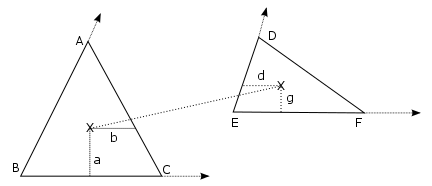
\includegraphics[width=0.3\textwidth]{sketches/c.png}
  \end{center}
  \caption{
    Triangle X:T1 (Vertices A, B, C) with barymetric parameters a,b that point $x$ point on the triangle. Triangle Y:T2 (D,E,F) with g,d parameters. The two barymetric points define the $P,Q$ points of the minimum distance between the two triangles in 3D.
  }
  \label{figure:barycentric_contact}
\end{figure}

\begin{equation}\label{eq:penalty}
P(x)=f(x)+r\sum_{i=1...6}max(0,c(x_{i}))^{2}
\end{equation}
Where r is the penalty parameter (figure \ref{figure:penaltyfunction}) that augments $f$. Convergence can be controlled by the r parameter that controls the sharpness of the constraint curve. One aspect that requires care however is the invertibility of the Hessian $\nabla\nabla P$ due to ill conditioning. This illustrates the fact that $f$ has multiple minima and $\nabla\nabla f$ is singular. Consequently, $\nabla\nabla P$ is also singular inside of the feasible region. The cause is due to multiple possible solutions when the orientation of the two triangles is parallel. This is also revealed by the two zero eigenvalues of the Hessian. We use a quasi-Newton approach, where the Hessian is approximated by a perturbation operator $\nabla\nabla P + \epsilon I$. $I$ is an identity matrix and $\epsilon$ is suitably small.

\begin{algorithmic}[1]
	
	\Function{Penalty}{A, B, C, D, E, F, rho, tol}

		\State $BA~=~B-A;~CA~=~C-A;~ED~=~E-D;~FD~=~F-D;$

		\State $hf~=~{[}2{*}BA{*}BA',~2{*}CA{*}BA',-2{*}ED{*}BA',-2{*}FD{*}BA';$

		\State $2{*}BA{*}CA',~2{*}CA{*}CA',-2{*}ED{*}CA',-2{*}FD{*}CA';$

		\State $2{*}BA{*}ED',-2{*}CA{*}ED',~2{*}ED{*}ED',~2{*}FD{*}ED';$

		\State $2{*}BA{*}FD',-2{*}CA{*}FD',~2{*}ED{*}FD',~2{*}FD{*}FD'{]};$

		\State $x~=~{[}0.33;~0.33;~0.33;~0.33{]};$

		\For{i=1:99}

			\State $X~=~A+BA{*}x(1)~+~CA{*}x(2);$

			\State $Y~=~D+ED{*}x(3)~+~FD{*}x(4);$

			\State $gf~=~{[}2{*}(X-Y){*}BA';~2{*}(X-Y){*}CA';~-2{*}(X-Y){*}ED';~-2{*}(X-Y){*}FD'{]};$

			\State $h~=~{[}-x(1);~-x(2);~x(1)+x(2)-1;~-x(3);~-x(4);~x(3)+x(4)-1{]};$

			\State $dh~=~{[}-1,~0,~1,~0,~0,~0;~0,~-1,~1,~0,~0,~0;$

			\State $0,~0,~0,~-1,~0,~1;~0,~0,~0,~0,~-1,~1{]};$

			\State $mask~=~h'~$>$=~0;$

			\State $dmax~=~dh.{*}~{[}mask;~mask;~mask;~mask{]};$

			\State $gra~=~gf~+~rho~{*}~dmax~{*}~max(0,h(:));$

			\State $hes~=~hf~+~rho{*}dmax{*}dmax'~+~eye(4,4)/rho^2;$

			\State $dx~=~hes\textbackslash{}gra;$

			\State $DX~=~BA{*}dx(1)~+~CA{*}dx(2);$

			\State $DY~=~ED{*}dx(3)~+~FD{*}dx(4);$

			\State $error~=~sqrt(DX{*}DX'+DY{*}DY');$

			\If{error~$<$~tol}
				\State $BREAK;$
			\EndIf

			\State $x~=~x~-~dx;$

		\EndFor

	\EndFunction
	
	%\caption{Penalty Solver.}
 	\label{algorithm:penalty}
\end{algorithmic}

The penalty algorithm as shown in Algorithm \ref{algorithm:penalty} accepts vertex coordinates for triangle T1(A, B, C), T2(D, E, F), $rho$ for the penalty parameter, and $epsilon$ for the perturbation, $tol$ is the tolerance error for convergence. At line 23 of Algorithm \ref{algorithm:penalty} an initial guess is set to be the center of the triangles, the For loop initiates the Newton solver to find the solution on the $X$, $Y$ triangle, under constraint c. For each constraint (line 12) the max function is evaluated to detect the active ones. At line 17 and line 18 the gradient and Hessian is evaluated for the Gaussian elimination direct solver (MATLAB backslash) to get $dx$ Newton direction

